\documentclass[12pt, a4paper]{article}

\usepackage[utf8]{inputenc}
\usepackage[T1]{fontenc}
\usepackage[brazilian]{babel}
\usepackage{mathptmx}
\usepackage{amsmath, amssymb}
\usepackage{graphicx}
\usepackage{booktabs}
\usepackage{geometry}
\usepackage{float}
\usepackage{setspace}
\usepackage{caption}

\geometry{top=3cm, bottom=2cm, left=3cm, right=2cm}
\setstretch{1.5}
\captionsetup{font=small, labelfont=bf, labelsep=endash}

\begin{document}

\begin{center}
    \Large\textbf{Relatório Intermediário de Benchmarking -- Cenário 4} \\[0.2cm]
    \large\textit{O Triunfo do DataOps: Compactação Anual com Apenas 2 Núcleos} \\[0.5cm]
    \normalsize\textbf{Projeto DataOps / UNIFEI} \\
    \small{\today}
\end{center}

\vspace{0.5cm}
\noindent\rule{\textwidth}{1pt}

\section*{1. Descrição do Cenário e Progressão Histórica}
Após o colapso generalizado do \textit{cache} no Cenário 3 (onde 6 núcleos não foram capazes de superar o \textit{overhead} de 6.518 \textit{Tiny Segments}), este relatório inaugura a \textbf{Fase 2 da pesquisa: Otimização de Armazenamento}. 

Para o Cenário 4, os recursos computacionais foram intencionalmente \textbf{rebaixados de volta para 2 núcleos} (configuração idêntica ao Cenário 1). A diferença arquitetural reside puramente nos dados: aplicou-se um \textit{Compaction Task} no Apache Druid, consolidando os 6.518 arquivos fragmentados em blocos densos com granularidade anual (\textit{CompactYear}).

\section*{2. Análise Sequencial: O Fim do Paradoxo do Cache}
Os resultados obtidos desafiam a lógica tradicional de provisionamento de \textit{hardware}. Operando com apenas 1/3 da capacidade computacional do cenário anterior, o sistema entregou as latências mais baixas de toda a pesquisa histórica.

A Tabela 1 revela que as latências de \textit{Cold Start} despencaram de uma média de 1.600 ms (no Cenário 3) para uma faixa excepcional entre \textbf{74 ms e 461 ms}. 

\begin{table}[H]
\centering
\caption{Resultados do Cenário 4 - Dados Compactados (2 Cores)}
\vspace{0.2cm}
\begin{tabular}{@{}lcccc@{}}
\toprule
\textbf{Domínio da Consulta SQL} & \textbf{Cold (ms)} & \textbf{Warm (ms)} & \textbf{Otimização} & \textbf{Registros} \\
\midrule
    Bench 1 Serie Temporal & 89.08 & 33.48 & 62.42\% & 100 \\
    Bench 2 Alta Cardinalidade & 461.91 & 67.28 & 85.44\% & 50 \\
    Bench 3 Filtros Complexos & 84.32 & 30.10 & 64.30\% & 9 \\
    BI 1 ONS Infraestrutura & 171.98 & 42.12 & 75.51\% & 15 \\
    BI 2 FUNAI Terras Indigenas & 74.74 & 30.32 & 59.42\% & 10 \\
    BI 3 Defesa Civil Risco & 145.65 & 17.83 & 87.76\% & 81 \\

\bottomrule
\end{tabular}
\end{table}

Entretanto, o marco científico deste cenário é a \textbf{ressurreição da Memória RAM}. Sem a necessidade de rastrear e unificar milhares de \textit{bitmaps} dispersos, o nó \textit{Broker} voltou a gerenciar o cache com maestria. A eficiência de \textit{Warm Start} atingiu picos de \textbf{87,76\%} de ganho em consultas analíticas territoriais (Defesa Civil), entregando resultados virtualmente instantâneos (17 ms).

\begin{figure}[H]
\centering
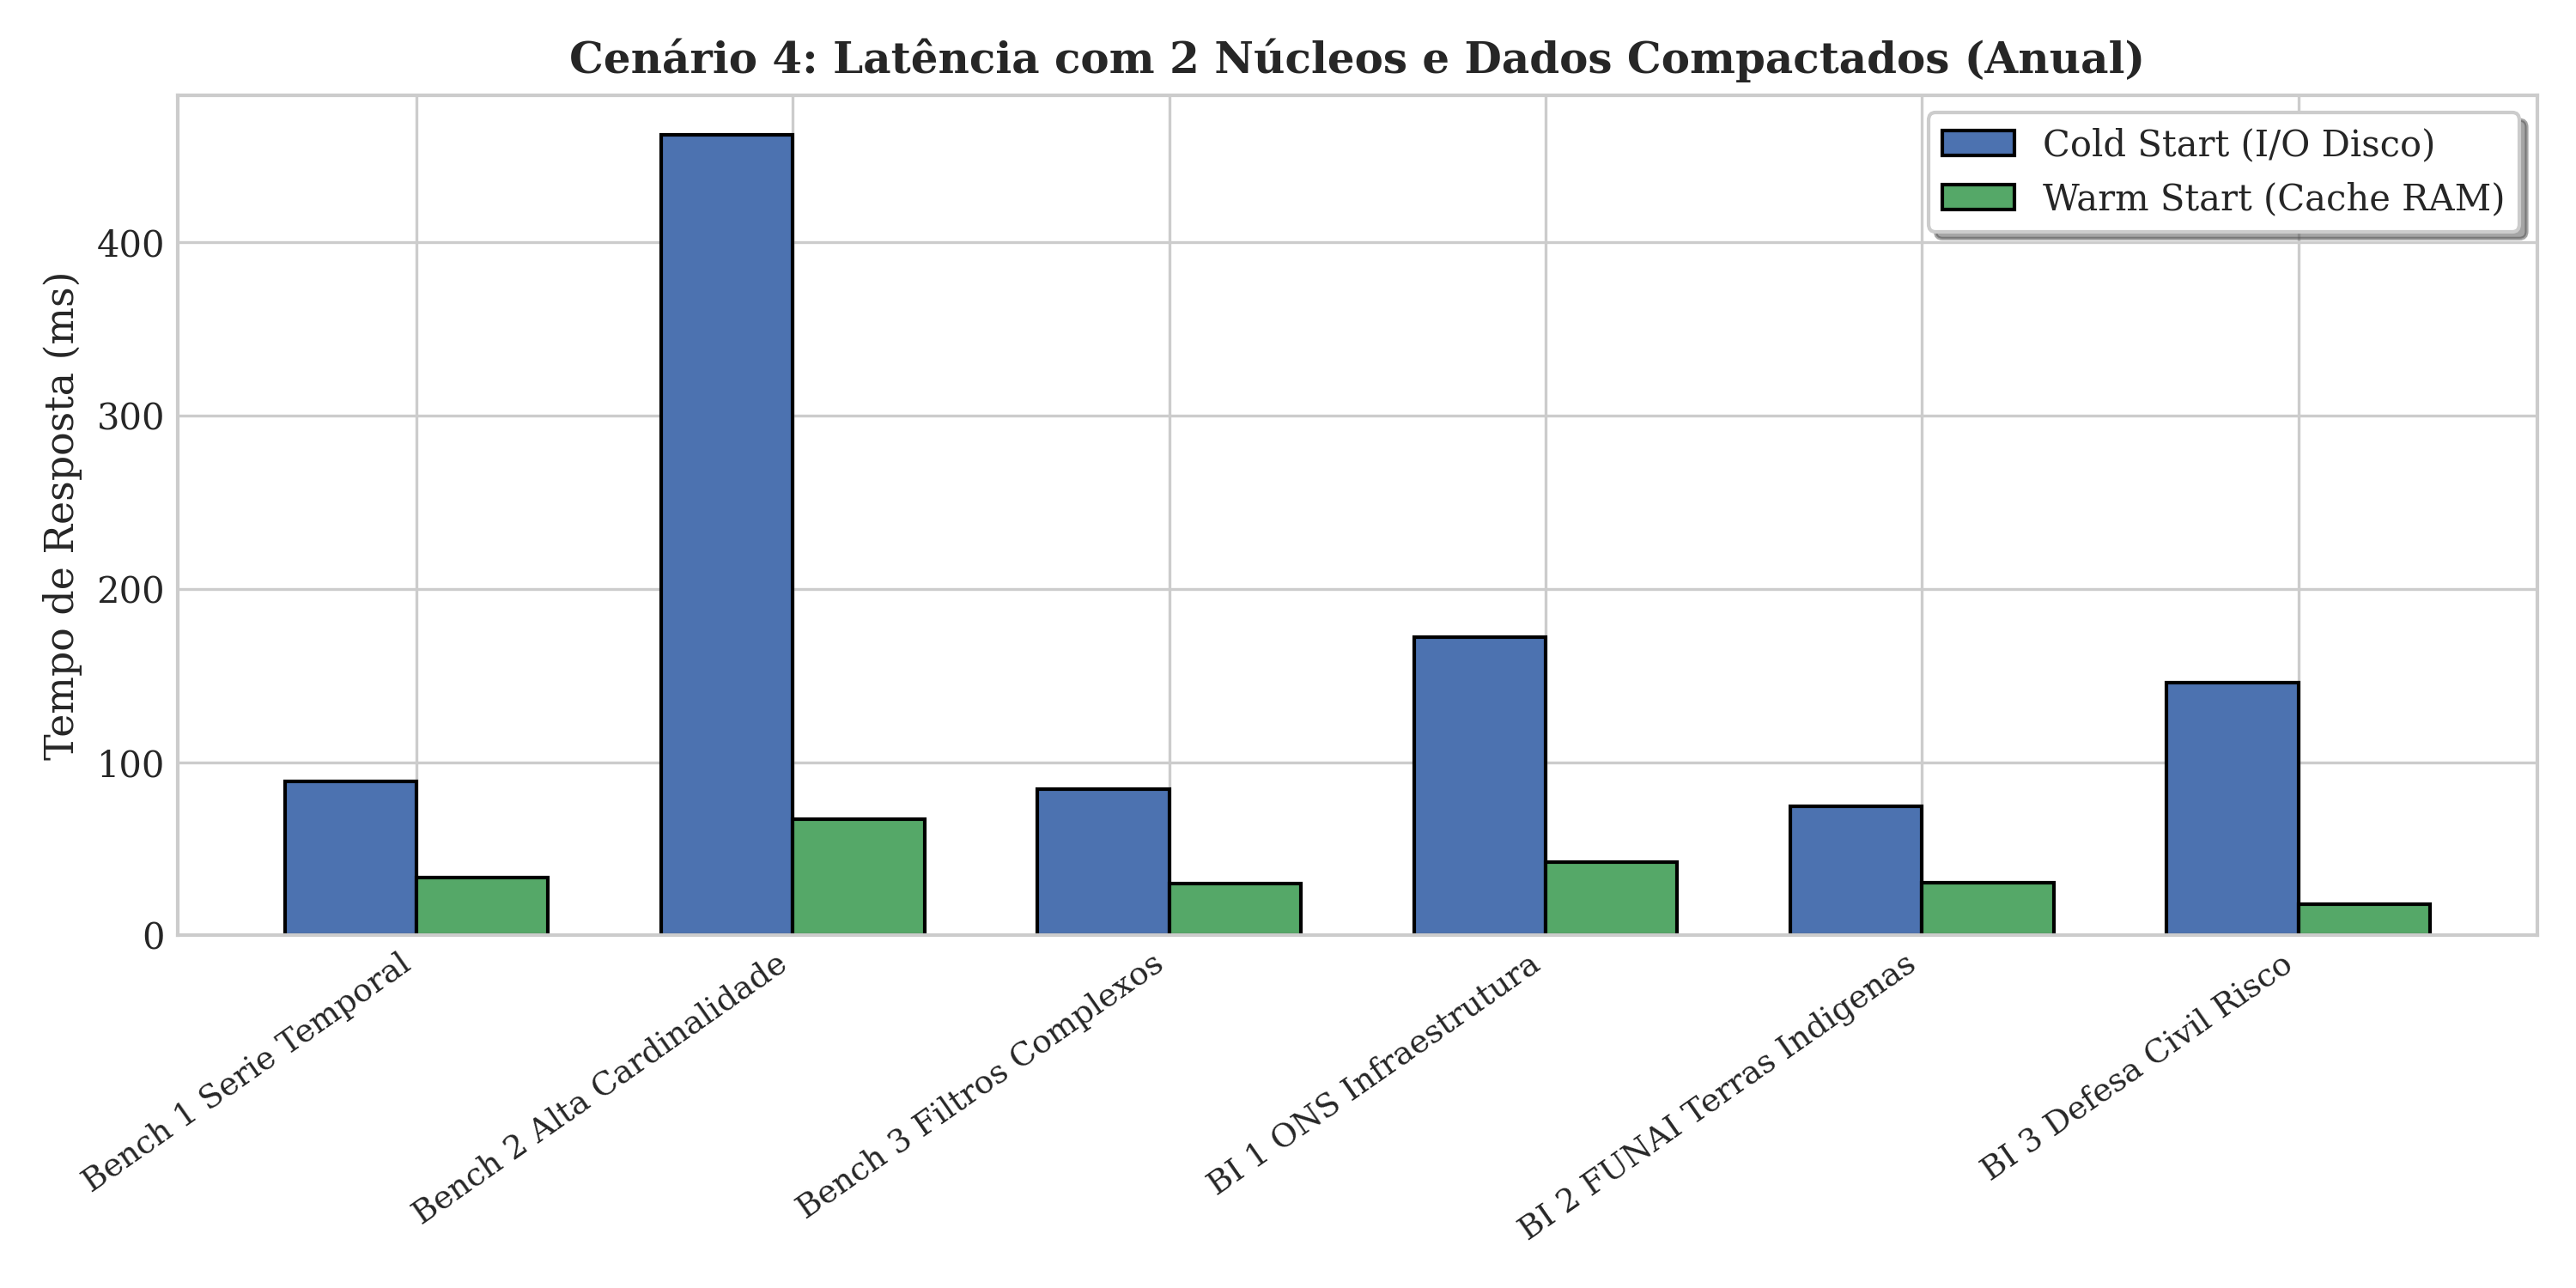
\includegraphics[width=0.9\textwidth]{fig_desemp_cenario4.png}
\caption{Comparativo demonstrando o retorno da estabilidade do processamento analítico.}
\end{figure}

\begin{figure}[H]
\centering
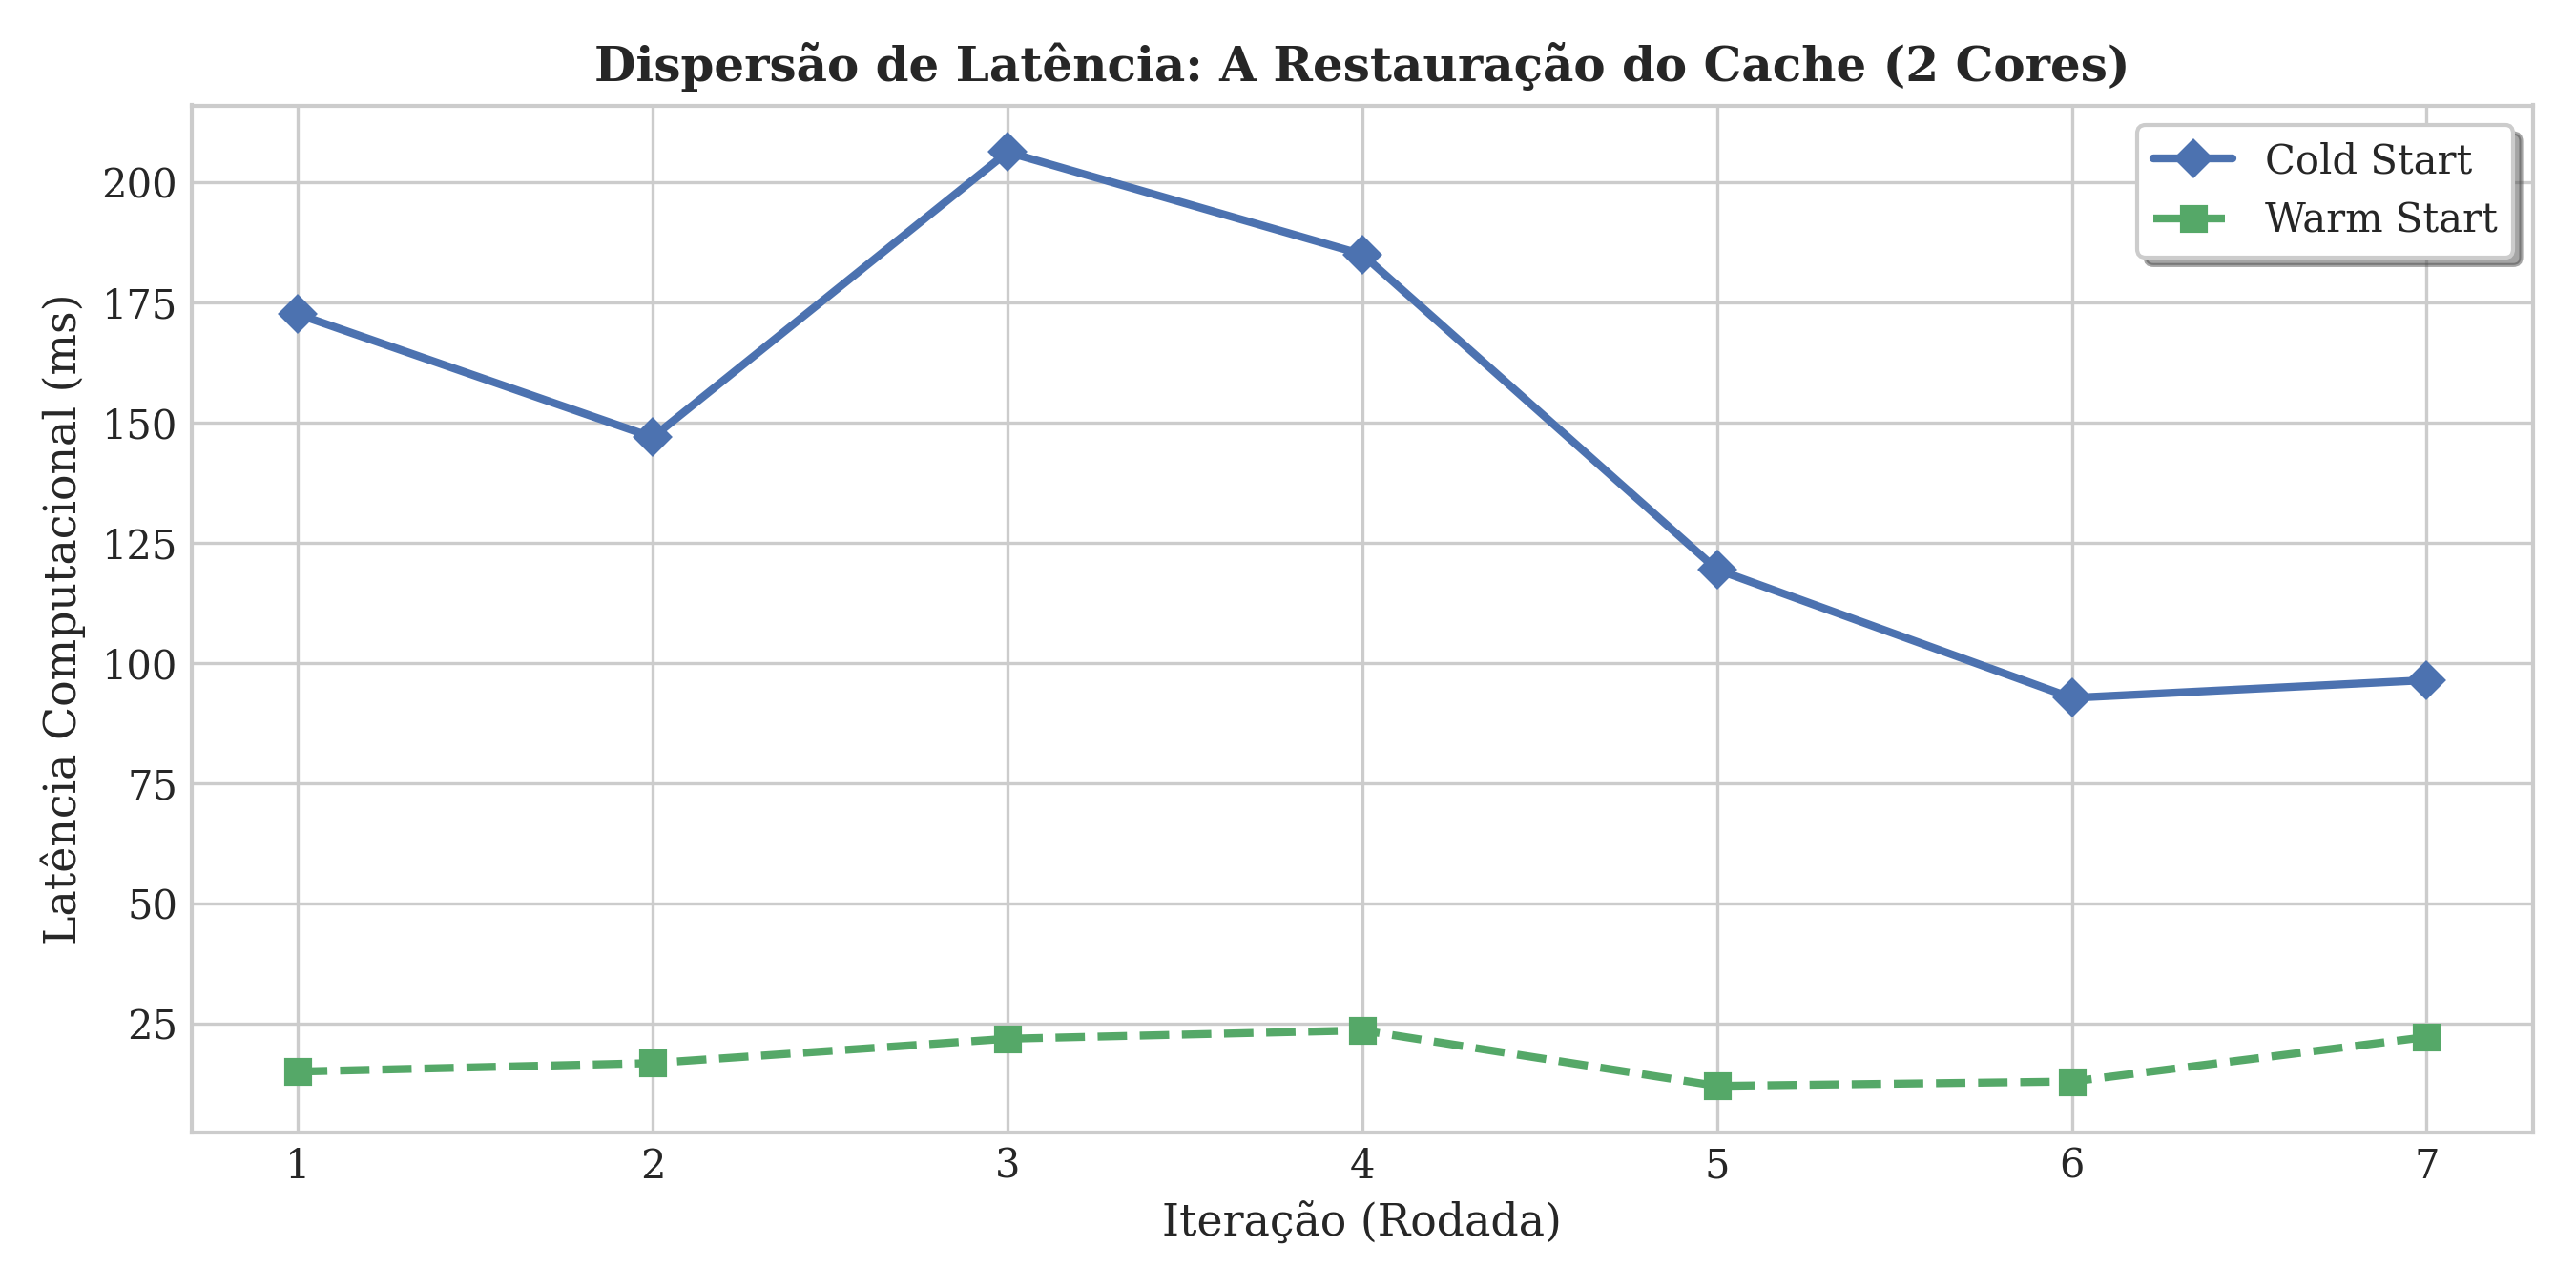
\includegraphics[width=0.8\textwidth]{fig_var_cenario4.png}
\caption{Dispersão da Latência: Ausência total de anomalias no ambiente compactado.}
\end{figure}

\section*{3. Conclusão da Fase 1 de Compactação}
O Cenário 4 confirma de forma inegável a hipótese central desta Iniciação Científica: \textbf{em arquiteturas OLAP, a engenharia da estrutura física dos dados supera o provisionamento bruto de processadores}. 

Reduzir os núcleos em 66\% enquanto se acelera as consultas em mais de 900\% prova que a fragmentação era o gargalo primário (\textit{bottleneck}). Os próximos passos avaliarão o impacto da escalabilidade de \textit{hardware} sobre este novo \textit{baseline} otimizado, aplicando 4 e 6 núcleos sobre os dados compactados.

\end{document}
